\documentclass[twocolumn]{cinc}
\usepackage{mathtools, graphicx, xurl, hyperref}
\usepackage{amssymb}
\usepackage{amsfonts}
\usepackage{booktabs}
\usepackage{xcolor}
% define macros
\newcommand{\jiaying}[1]{\textcolor{orange}{[jiaying: #1]}}

\title{Ensemble Learning with Early Fusion of Kernel-Transformed and Classical Electrocardiogram Features for Chagas Disease Detection}
\author{Victor Li,
Runze Yan,
Saurabh Kataria,
Alex Fedorov,
Jiaying Lu \\ \ \\
Emory University, Atlanta, GA, USA \\} 

\begin{document}
\maketitle

% Instruction: https://moody-challenge.physionet.org/2025/papers/cinc_template.pdf
% 4 pages for everything

%%%%%%%%%%%%%%%%%%%%%%%%%%%%%%%%%%%%%%%%%%%%%%%%%%%%%%%%%%%%%%%%%%%%%%%%%%%%%%%%

\begin{abstract}
The electrocardiogram (ECG) offers an accessible and non-invasive assessment of human health. Chagas disease, which affects nearly 6.5 million people across Central and South America, is known to have symptoms that appear in ECGs. Using time-series machine learning techniques, critical information can be extracted from these ECGs to detect Chagas disease as opposed to serological tests.

As part of the George B. Moody PhysioNet Challenge 2025, we developed a classification approach consisting of two components: (1) dense representation of 12-lead ECGs; (2) ensemble classification. Our team, GAIN-ECG, developed a novel approach that combines kernel-based feature extraction through MiniRocket with classical signal features, such as Heart Rate Variability (HRV), Continuous Wavelet Transform (CWT), and Fast Fourier Transform (FFT) features, through early fusion. We then employ an ensemble framework to classify the onset of Chagas disease.

Testing against a held-out subset of the public training set, our model achieved a challenge score of 0.481, AUROC of 0.880, and F1 of 0.113. However, these results aren't comparable to official challenge scores because of the large differences between the training, validation, and test sets. As a result, on the hidden validation set, our model achieved a challenge score of 0.090.

\end{abstract}

%%%%%%%%%%%%%%%%%%%%%%%%%%%%%%%%%%%%%%%%%%%%%%%%%%%%%%%%%%%%%%%%%%%%%%%%%%%%%%%%

\section{Introduction}
As team GAIN-ECG, we participated in the 2025 George B.\ Moody PhysioNet Challenge. This challenge invited teams to develop automated and open-sourced algorithms for classifying cases of Chagas from eletrocardiograms (ECG) \cite{Goldberger2000, 2025Challenge}. Although ECG-based diagnoses of Chagas disease can often be inaccurate, they can inform the use of limited and invasive serological tests. 

Our team's Challenge entry tackles this classification task through a novel two-part approach utilizing dense representations of 12-lead ECGs and ensemble learning. The core of our approach lies in feature engineering and extraction. Assuming high performance can be achieved by our downstream classifier, our model’s performance hinges on the richness and reliability of the features. 

Training and validating on the Challenge's public training set and hidden validation set \cite{CODE-15, SaMi-Trop, PTB-XL, REDS-II, ELSA-Brasil}, we found that cross-ECG machine batch effects significantly undermined the reliability of our feature extraction process. To address this, we utilize classical signal features that directly capture ECG-specific characteristics, rather than relying on pretrained foundation models, which risk encoding batch-dependent features that worsen performance when evaluated on unseen batches. Also, we implement a convolutional kernel-based encoder to extract additional features, which are incorporated with early fusion.

%%%%%%%%%%%%%%%%%%%%%%%%%%%%%%%%%%%%%%%%%%%%%%%%%%%%%%%%%%%%%%%%%%%%%%%%%%%%%%%%
% final best model had no data weight and no z-score norms

\section{Methods}
Our two-stage multi-view ensemble classification framework consist of two key components: (1) multi-view ECG representation learning, and (2) ensemble classifier. The multi-view representation learning module~\cite{Kataria2025PPGFMCA} is designed to capture the characteristics of input ECG signals from multiple, complementary perspectives. The ensemble classifier follows a similar principle, leveraging diverse base classifiers with different inductive biases to enhance predictive performance.

As shown in Figure~\ref{model figure}, our framework begins by extracting classical features from three different views: Heart Rate Variability~\cite{hrv} (HRV), Discrete Wavelet Transform~\cite{wavelet} (CWT), and Fast Fourier Transform~\cite{fft} (FFT). Alongside these classical features, we also extract kernel-based representations of the ECG signals through MiniRocket~\cite{minirocket}, a convolutional kernel-based encoder. The extracted classical and kernel-based features are then integrated via early fusion, where all features are concatenated to dense vectors. In the second stage of our approach, these dense features are used to train an ensemble of classifiers, such as tree-based models, boosting models, tabular neural networks, and K-Nearest Neighbors (KNN). These models are optimized under the AutoGluon~\cite{autogluon} automated machine learning framework.

\begin{figure}[htbp!]
    \centering
    \includegraphics[width=1.0\linewidth]{model.png}
    \caption{\textbf{Overview of proposed framework}. Every ECG signal is first processed through the feature extractors in the first component to create dense vector representations. Then, Chagas diagnosis is determined by an ensemble classifier in the second component.}
    \label{model figure}
\end{figure}

\subsection{Multi-view ECG Representation Learning}
We denote one raw input 12-lead 400Hz ECG record as $\mathbf{x}\in \mathbb{R}^{L\times T}$, where $L=12$ and $T$ is originally variable depending on the record length (\textit{e.g.}, 7 seconds, 10 seconds). To maintain consistency across samples, each signal is either truncated or zero-padded to a fixed length of $T=4096$. 

\jiaying{I will probably put this before the ensemble classifier.} In addition, we calculate the means and standard deviations of each individual ECG lead, which are then fused with the classical kernel-based features through concatenation.

\noindent \textbf{Heart Rate Variability Representation}
We opt HRV as one view of ECG representation, which quantifies the variation in time intervals between consecutive heartbeats.
% assume you are using the package: NeruoKit2
To extract the HRV features, we first detect R-peaks in each ECG record (the tallest spikes in the QRS complex). This is achieved by finding  a set $\mathbf{C}$ of all local-maxima in the Lead II of ECG record $\mathbf{x}^{(2)}\in \mathbb{R}^T$:
\begin{equation}
    \begin{aligned}
        \mathbf{C} = \{t & \in \{2, \dots, T-1\}: \\
        & x^{(2)}[t-1]<x^{(2)}[t]>x^{(2)}[t+1]\}.
    \end{aligned}
    \label{peaks}
\end{equation}
To ensure the plausibility of our peaks, we enforce a minimum distance of 200 ms between consecutive peaks, which corresponds to a maximum heart rate of 300 bpm. R-peaks are then greedily selected from $C$ under this constraint. %To maintain consistent feature dimensionality across signals, we do not use the raw R-peak locations directly. Instead, we derive several summary representations. 
Based on the obtained R-peaks, we derive the following time-domain HRV features: (1) mean RR intervals ($\bar{\text{RR}}$) that capture the beat-to-beat timing; (2) Standard Deviation of RR intervals (SDNN) that reflects overall heart rate variability; (3) Root Mean Square of Successive Differences (RMSSD) that emphasizes short-term variability between consecutive beats. The sequence of RR intervals are obtained by $RR_i=\mathbf{C}_{R_{i+1}}-\mathbf{C}_{R_i}$,
where $\mathbf{C}_{R_{i+1}}$ denotes the time of the i-th R-peak in $\mathbf{C}$. Therefore, we obtain HRV view representation as $\mathbf{h}_{\text{HRV}}=\bar{\text{RR}}\oplus \text{SDNN} \oplus \text{RMSSD}$.

% Therefore, 
% \begin{equation}
%     \bar{\text{RR}}=\frac{1}{\lvert \mathbf{C} \rvert}\sum_{i}^{\lvert \mathbf{C} \rvert}\text{RR}_i,
% \end{equation}
% \begin{equation}
%     \text{SDNN}= \text{to be done...},
% \end{equation}

%The number of R-peaks provides a coarse measure of overall heart rate over the signal duration. The average RR-intervals, computed as the average of the time differences between successive R-peaks, capture the beat-to-beat timing. From these intervals, we calculate the Standard Deviation of Normal-to-Normal intervals (SDNN), which reflects overall heart rate variability, and the Root Mean Square of Successive Differences (RMSSD), which emphasizes short-term variability between consecutive beats.



\noindent \textbf{Discrete Wavelet Transform Representation}
Using \textit{PyWavelets}, we decompose each ECG signal with a Daubechies-4 (db4) wavelet across four levels. The decomposition yields one approximation coefficient set and multiple detail coefficient sets. We ignore the approximation coefficients and compute the energy of each detail level by summing the squared values of its coefficients. These features capture the power of oscillations across 4 different frequency scales.


\noindent \textbf{Fast Fourier Transform Representation}
Lastly, to extract the FFT features, we first subsample signals down to 200 points to reduce computational complexity. Applying the FFT to the signal, we compute a set of complex coefficients $B[i]$ and their corresponding frequency bins $f_i$. Since ECG signals are real-valued, their FFTs are symmetric about zero, and we retain only the non-negative frequencies. The amplitudes $A_i$ are then computed as the normalized magnitude of $B[i]$, scaled by a factor of $2/N$ to account for the symmetry as shown in Equation~\ref{fft}. These features capture the larger and more dominant oscillatory components of the ECG signals that might be overlooked by R-Peaks statistics and wavelet energies.

\begin{equation}
    A_k = \frac{2}{N} \cdot \left| B[i] \right|, \quad \text{for } f_i \geq 0
    \label{fft}
\end{equation}

\noindent \textbf{Convolutional Kernel-based Representation}
To obtain kernel-based view of ECG signals, we implement a convolutional kernel-based MiniRocket encoder. Our encoder applies a fixed set of convolutional kernels to each univariate signal, each parameterized by a combination of dilation and bias quantile values. The outputs for the 12 leads are aggregated in the end. Unlike traditional learned convolutional networks, the kernels in MiniRocket are predetermined, which makes the transform extremely efficient.

We configure the encoder with 504 kernels, which correspond to MiniRocket’s base set of 84 kernels applied across 6 different dilations. Each kernel is convolved with the ECG signal, and the resulting outputs are converted into binary features by comparing them against pre-specified bias quantiles computed from the training data. Rather than storing the raw convolution outputs, MiniRocket summarizes them using the Proportion of Positive Values (PPV) statistic. The PPV measures the fraction of time points where the convolution response exceeds its bias threshold. For a signal $x$ with kernel $k$ at dilation $d$ for the bias quantile $b_{k,d}$, its PPV yields a binary value following Equation~\ref{ppv}.

\begin{equation}
    \text{PPV}_{k,d} = \frac{1}{T} \sum_{t=1}^{T} 1( (x * k_d)[t] > b_{k,d} )
    \label{ppv}
\end{equation}

Each kernel captures local patterns in the ECG signal at different temporal resolutions, while the bias quantile values allow the encoder to distinguish meaningful activations from background noise. By combining many PPVs across kernels and dilations, MiniRocket generates features that are most robust against batch variation.

\subsection{Ensemble Classifier}
From the multi-view ECG representation learning, we obtain the final dense vector $\mathbf{h}=\mathbf{h}_{\text{HRV}}\oplus \mathbf{h}_{\text{DWT}}\oplus \mathbf{h}_{\text{FFT}}\oplus \mathbf{h}_{\text{ConvK}}$. 
%para1: introduce each of the weak classifier
For our classification task, we implement the state-of-the-art tabular predictor in \textit{AutoGluon@1.3.0}. This classifier ensembles together a diverse set of models to make predictions, including tabular neural networks, tree-based, boosting-basde, and K-Nearest Neighbors (KNN) models. We configured AutoGluon to the "best quality" preset and impose a 24-hour time limit on training. During training, models are fit sequentially and subsequently ensembled into layers, with their weights determined based on performance on held-out subsets of the training data, using the official challenge evaluation metric.

% para2: introduce the weighted ensemble layer to produce the final result
% if someone can help write the bagging part.
% maybe add a figure. 

%%%%%%%%%%%%%%%%%%%%%%%%%%%%%%%%%%%%%%%%%%%%%%%%%%%%%%%%%%%%%%%%%%%%%%%%%%%%%%%%

\section{Results}
\subsection{Phase 1 Results}

\subsection{Ablation Study}
Using the publicly available training set, we performed an ablation study to track the benefit of each component we added to our model. We first started with a basic random forest on signal means and standard deviations. Second, we incorporated the kernel-transformed features from MiniRocket. Third, we switched the classifier from random forest to AutoGluon’s ensemble framework. Fourth, we added the classical signal features. Fifth, we incorporated data weights, where the weak data from the CODE-15\% dataset only contributed a tenth as much as the strong datasets to the loss function. Sixth, we incorporated z-score normalization on individual ECGs.

From the chart, we can see that the fifth variant of our model performed the best on the public training set. However, results from the hidden validation set indicates that the data weights actually worsen performance. We can also see that the overall performance of our model on the hidden validation set is much worse than the performance on a held-out subset of the training set. We believe this suggest that our model is overfitting to the differences between the datasets, rather than the chagas disease itself. The increases in performance with the addition of more classical features that are less prone to batch-effect indicate this as well.

In conclusion, we hope to briefly account for batch-effect using the signal based z-score normalization. We saw small improvements with this addition, once again demonstrating the significance of batch-effect in this competition. Ultimately, we felt our model could be improved much further with stronger feature engineering techniques focused on batch-effect removal.
%%%%%%%%%%%%%%%%%%%%%%%%%%%%%%%%%%%%%%%%%%%%%%%%%%%%%%%%%%%%%%%%%%%%%%%%%%%%%%%%

\section{Discussion and Conclusions}

%%%%%%%%%%%%%%%%%%%%%%%%%%%%%%%%%%%%%%%%%%%%%%%%%%%%%%%%%%%%%%%%%%%%%%%%%%%%%%%%

\section*{Acknowledgments}  
This work was supported in part by the Emory Undergraduate Research Programs and the Nell Hodgson Woodruff School of Nursing Center for Data Science of Emory University.
%%%%%%%%%%%%%%%%%%%%%%%%%%%%%%%%%%%%%%%%%%%%%%%%%%%%%%%%%%%%%%%%%%%%%%%%%%%%%%%%

\bibliographystyle{cinc}
\bibliography{references}

\begin{correspondence}
Jiaying Lu, PhD\\
1520 Clifton Road, Suite 245, Atlanta, GA 30322, USA\\
jiaying.lu@emory.edu
\end{correspondence}

\balance

\end{document}